
\subsection{Noveno sprint de producción}

Esta etapa contiene el desarrollo del nivel noveno del juego. El panorama general abarca un nivel de manera horizontal en un terreno oscuro. Después se llega al jefe enemigo Nexoxcho.

Primero se empieza con el maquetado del nivel, para establecer el tamaño del nivel, el nivel es de manera horizontal. Se establece también donde debe ir cada objeto o enemigo junto con anotaciones necesarias para la comprensión posterior, como son direcciones de movimiento o acciones que deben realizarse. Se cuenta con diferentes intercambios de escena ya que en esta ocasión se usa otro personaje para el jugador. Lo anterior se puede ver en la figura \ref{fig:n901}.
\begin{figure}[htbp]
	\centering
	\subfigure[Primera parte del nivel]{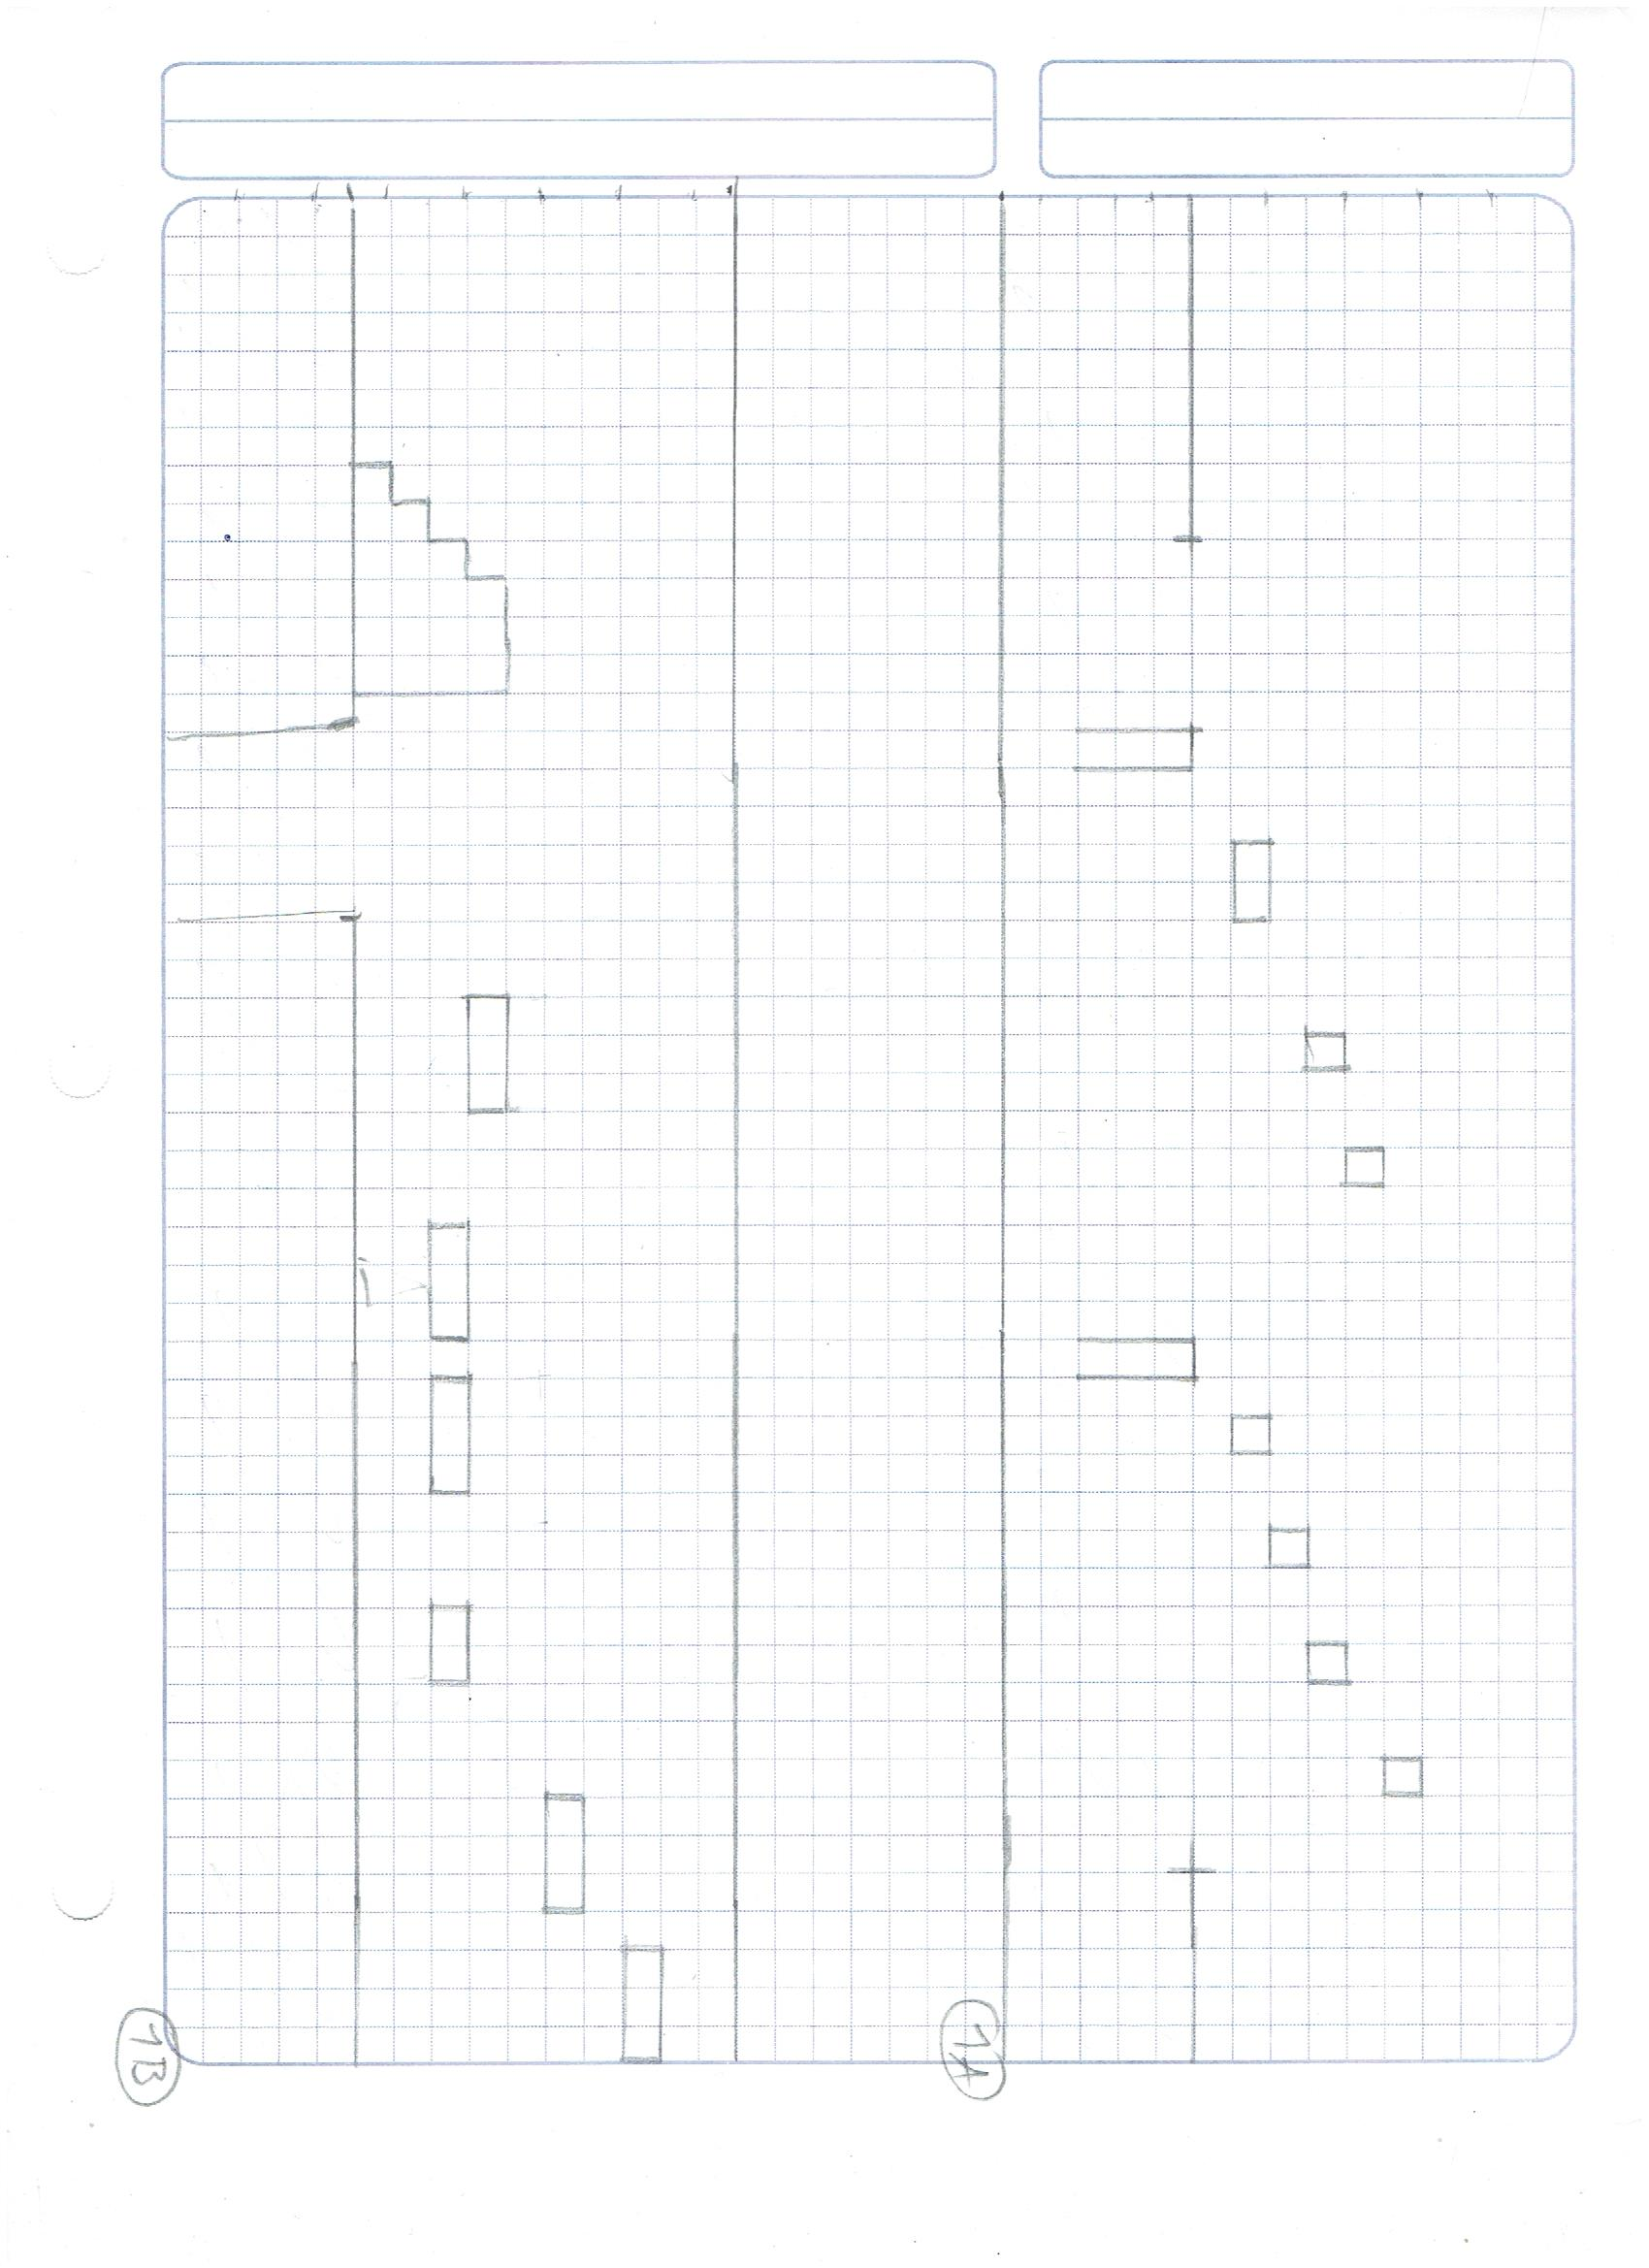
\includegraphics[width=5cm]{03TrabajoRealizado/DocProduccionR/imagenes/n9/13.jpeg}}
	\subfigure[Segunda parte del nivel]{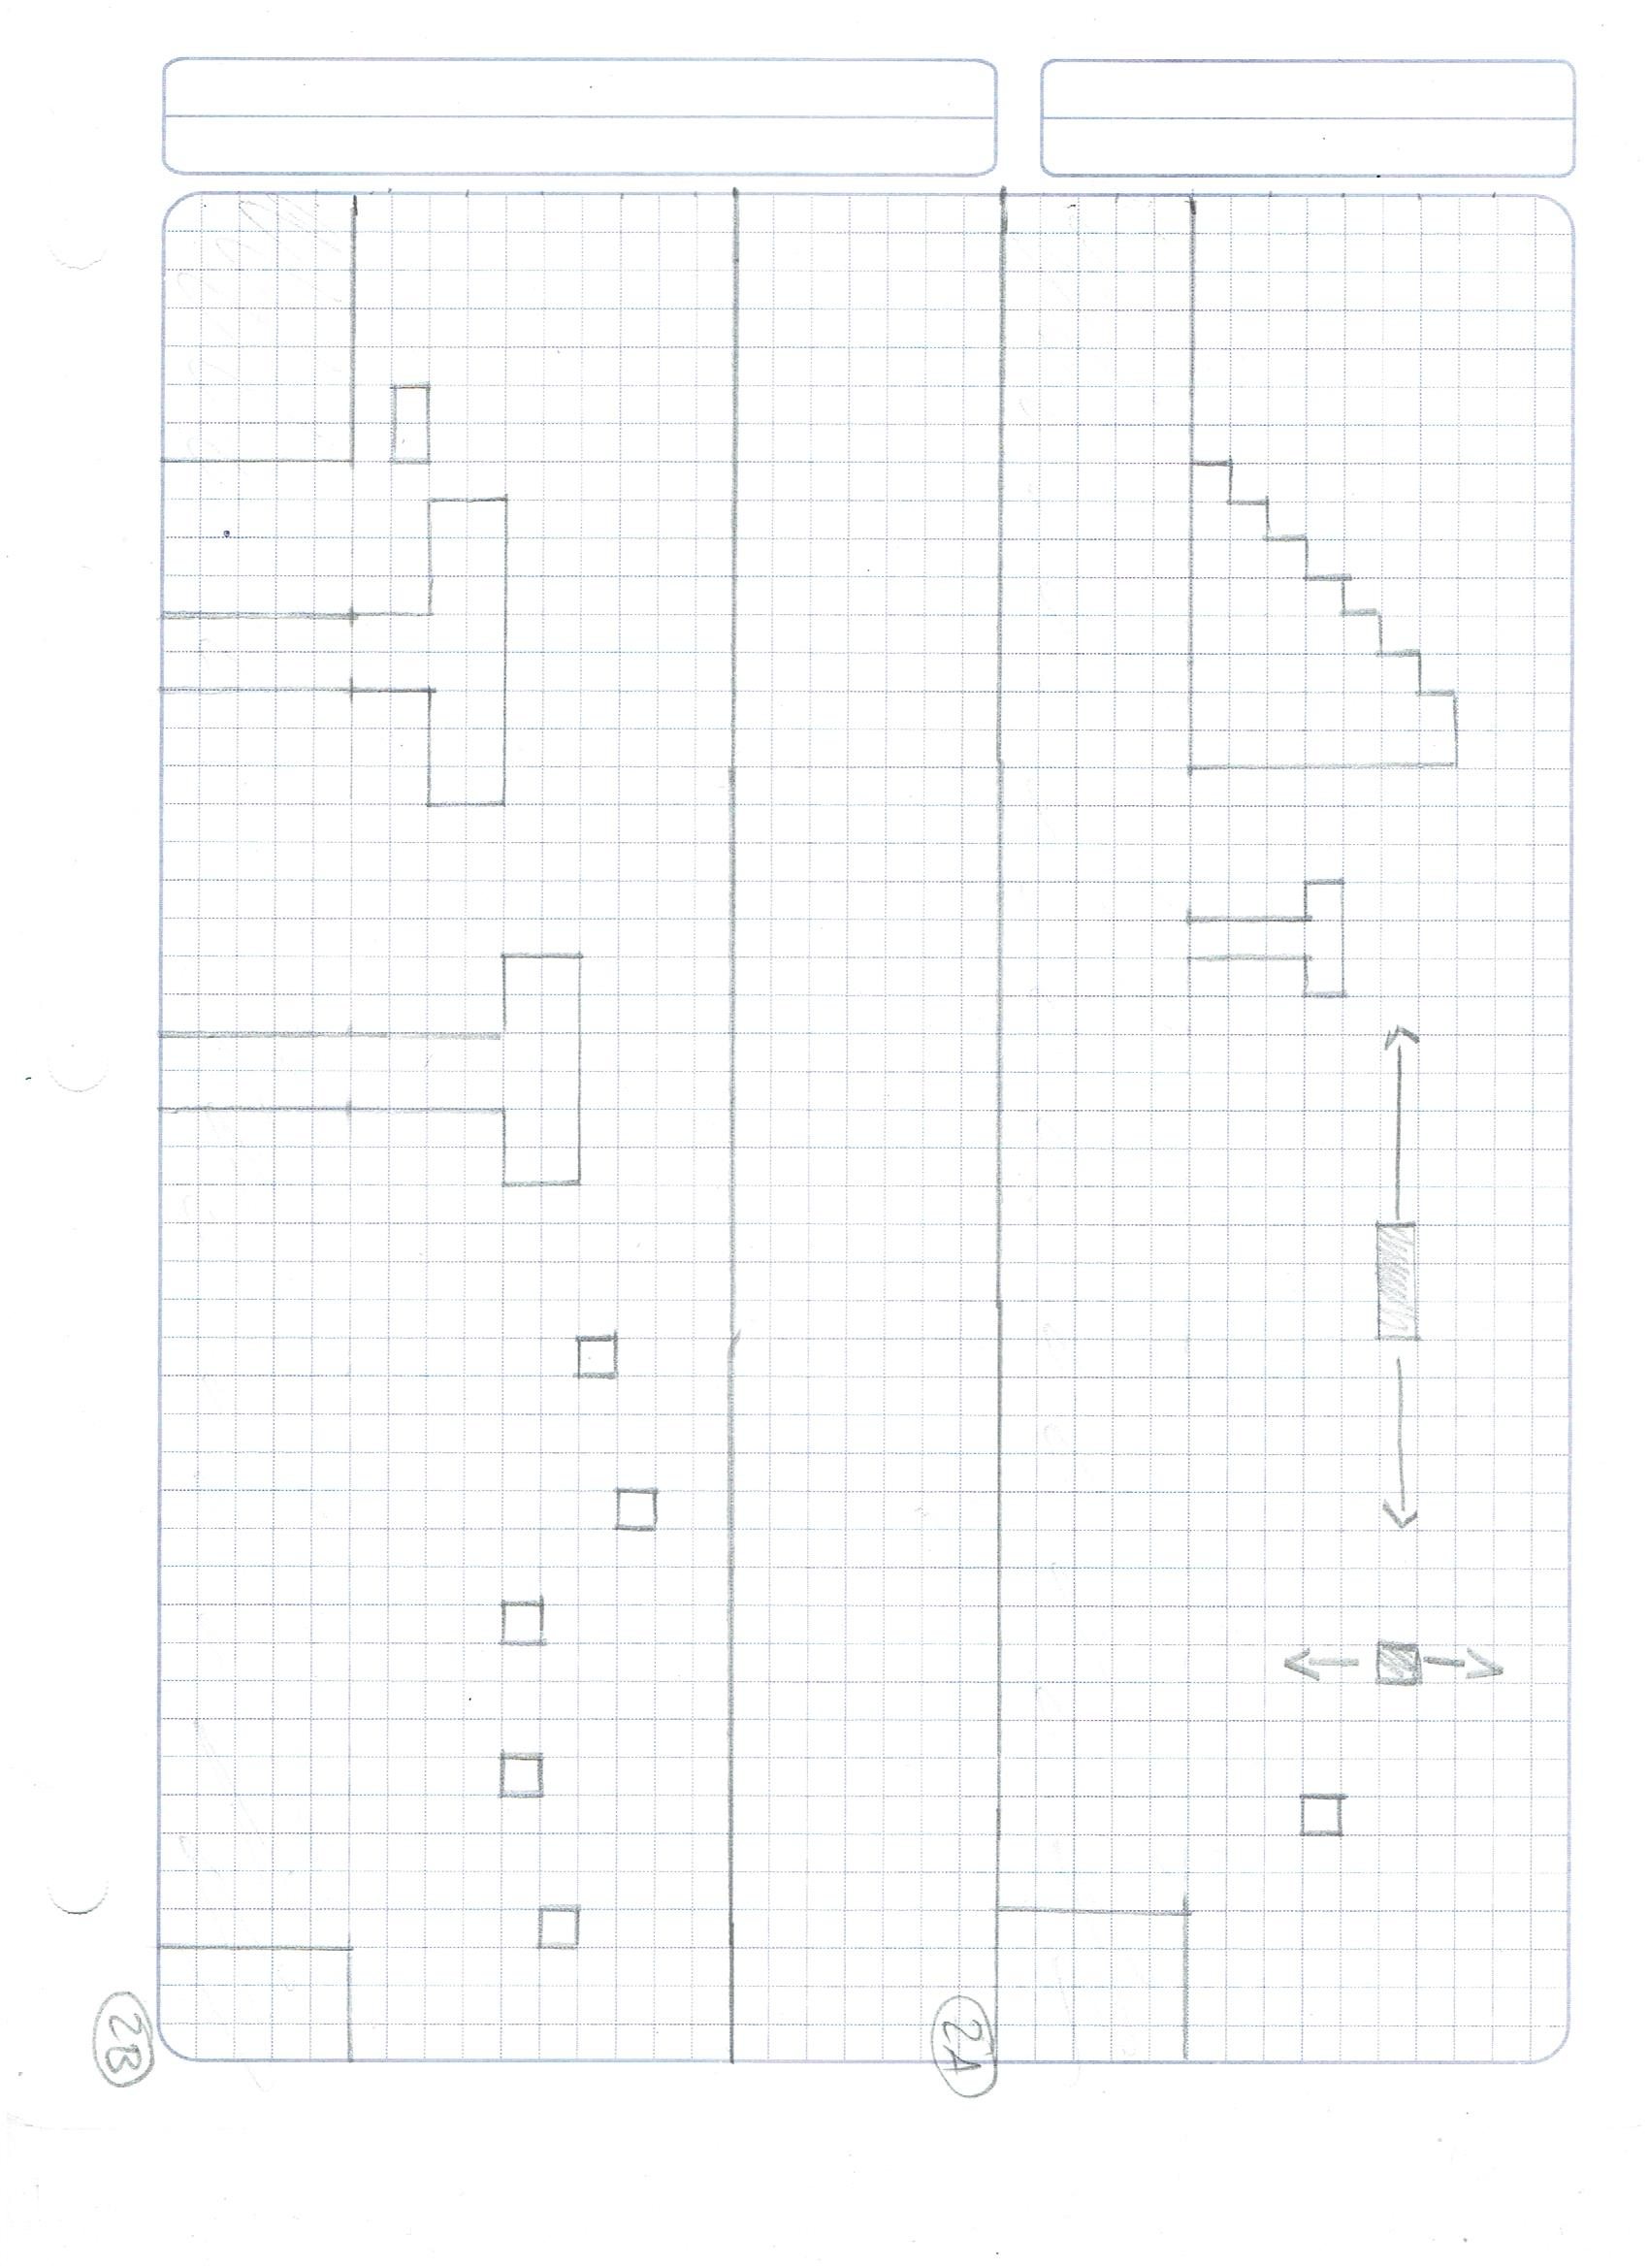
\includegraphics[width=5cm]{03TrabajoRealizado/DocProduccionR/imagenes/n9/14.jpeg}}
	\subfigure[Tercera parte del nivel]{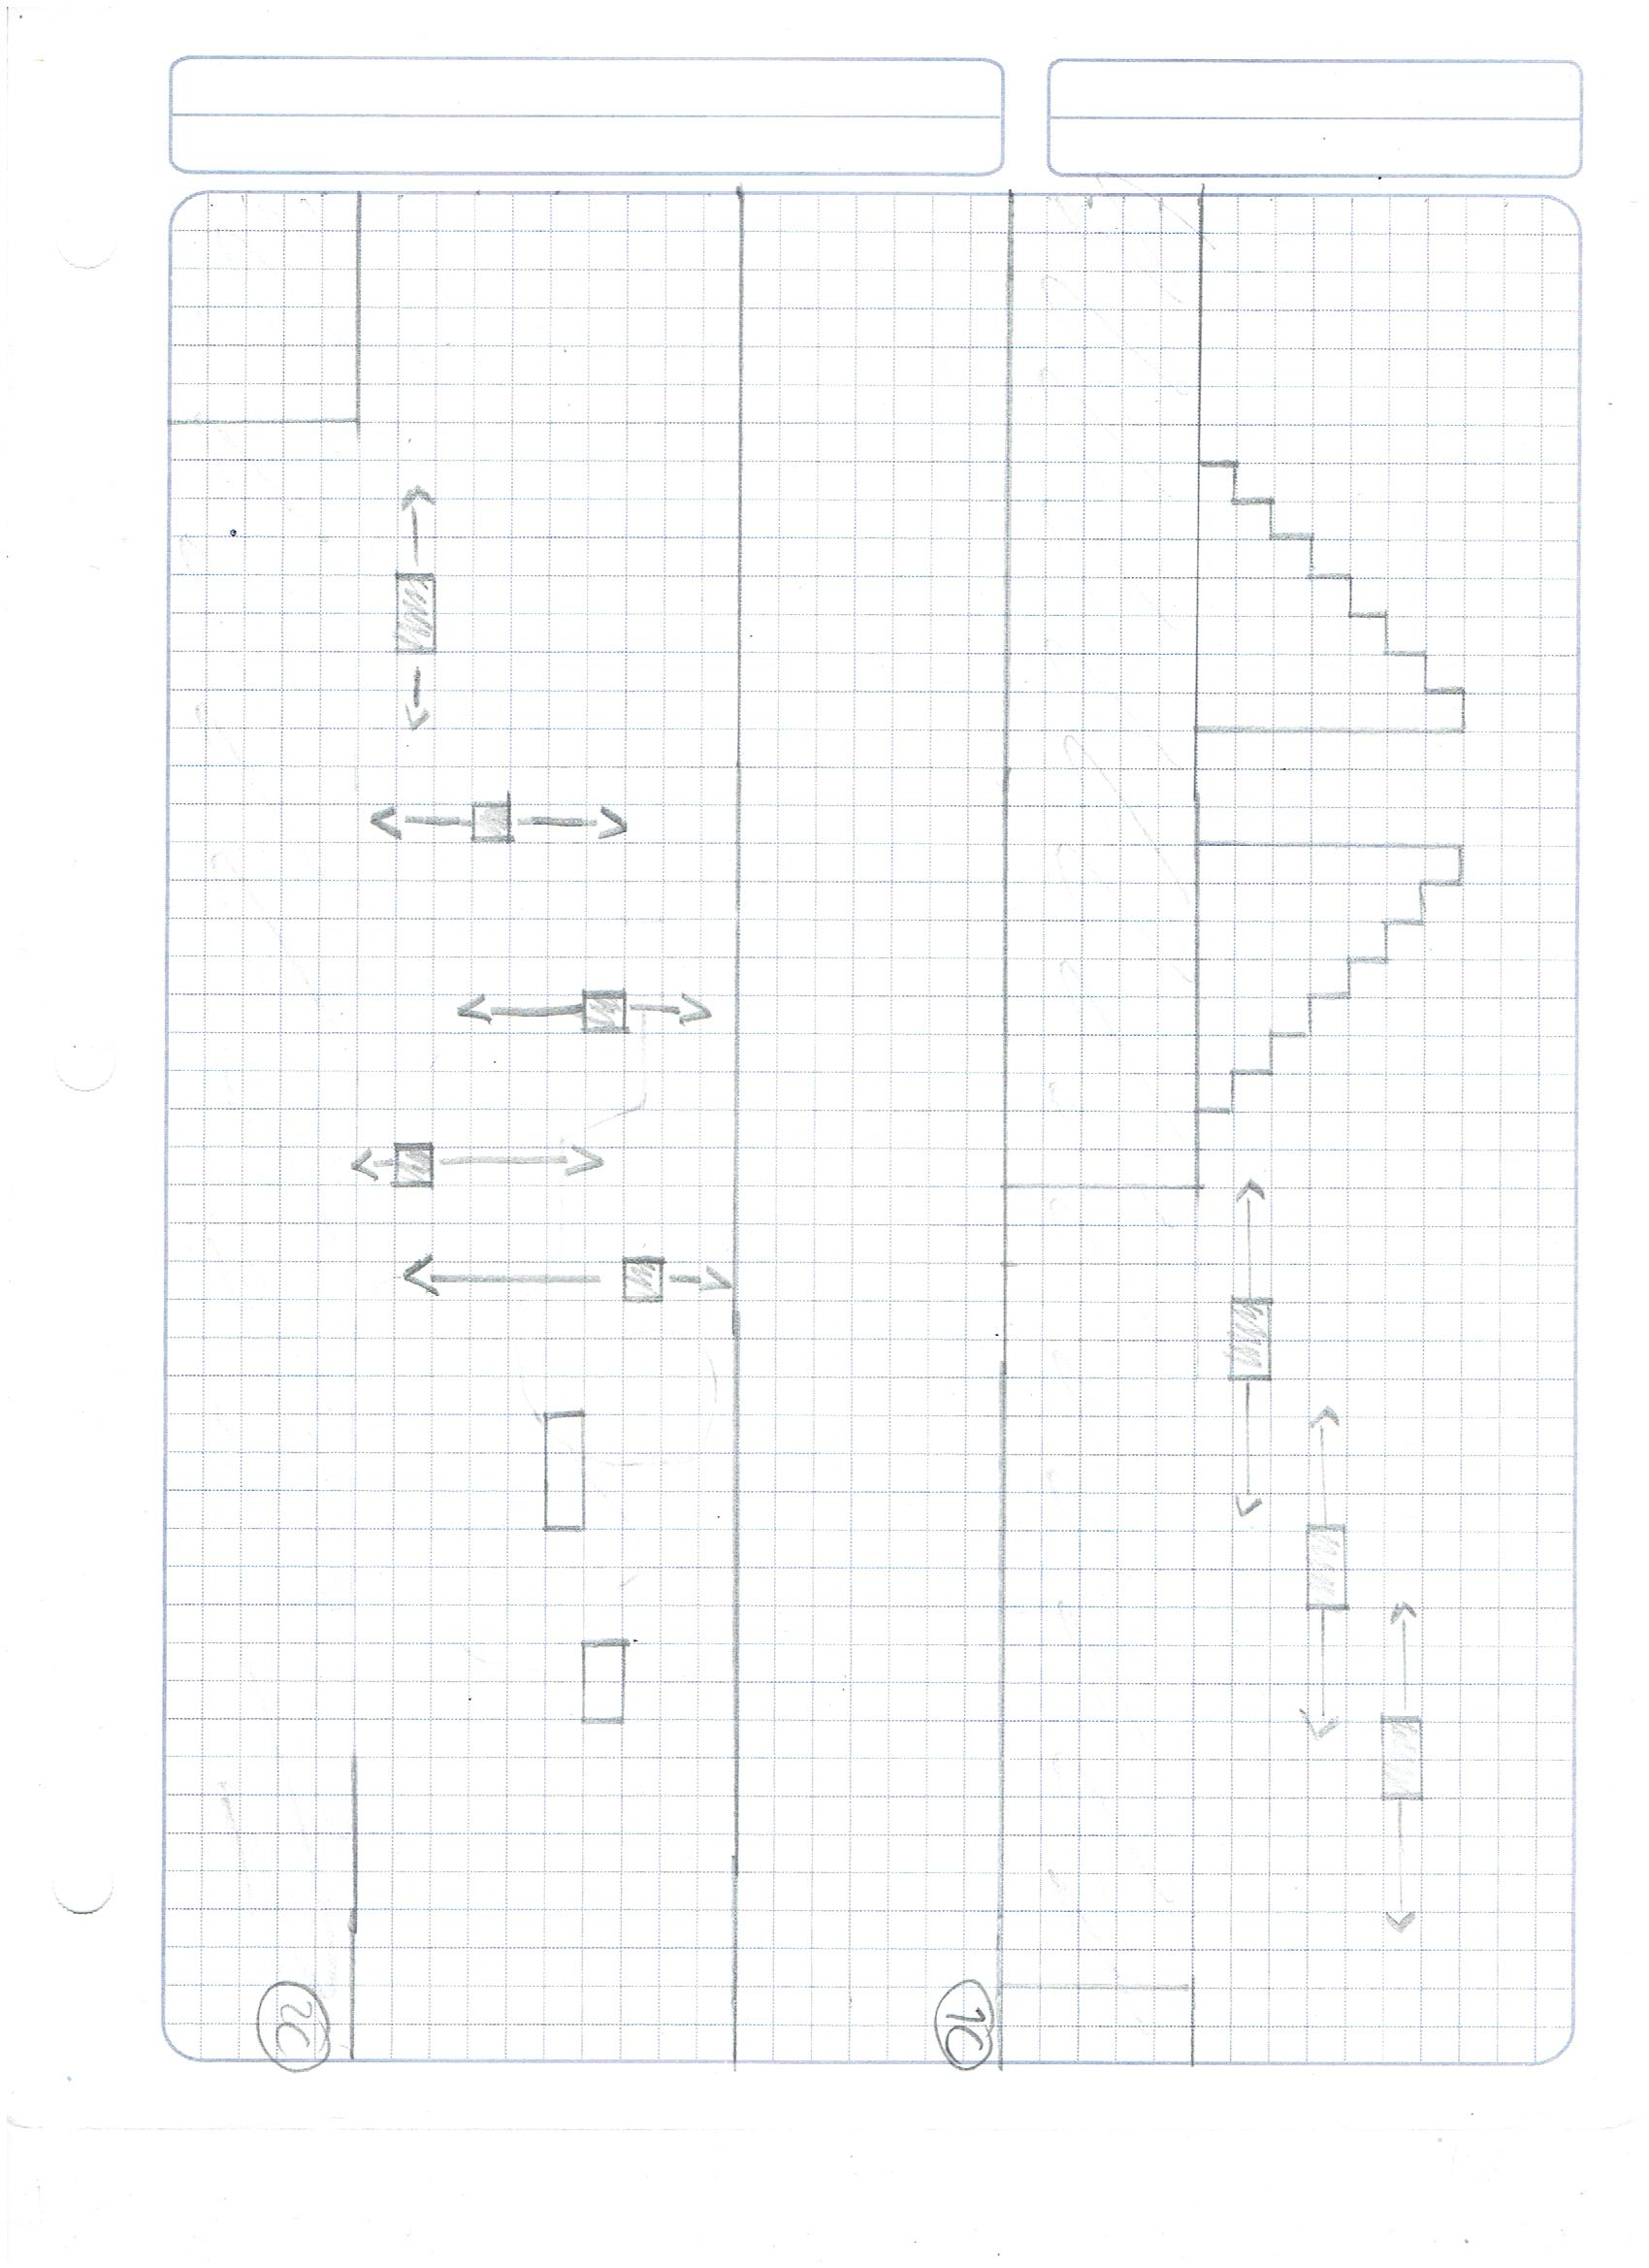
\includegraphics[width=5cm]{03TrabajoRealizado/DocProduccionR/imagenes/n9/15.jpeg}}
	\caption{Maquetado de nivel nueve} \label{fig:n901}
\end{figure}  

Después se lleva la tarea de tomar todos los componentes solo de manera visual y adecuar el tamaño necesario, tomando en cuenta las medidas de los componentes anteriores. Dichas imágenes se pueden ver en la \ref{fig:n902}.
\begin{figure}[htbp]
	\centering
	\subfigure[Imagen Xolotl y Malinalli.]{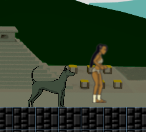
\includegraphics[width=5cm]{03TrabajoRealizado/DocProduccionR/imagenes/n9/n901.png}}
	\subfigure[Imagen de jefe enemigo Nexoxcho.]{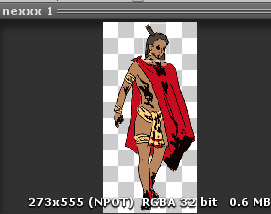
\includegraphics[width=5cm]{03TrabajoRealizado/DocProduccionR/imagenes/n9/n903.png}}
	\subfigure[Imagen de cara de jefe enemigo.]{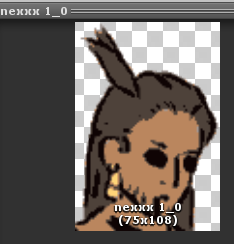
\includegraphics[width=5cm]{03TrabajoRealizado/DocProduccionR/imagenes/n9/n904.png}}
	\subfigure[Imagen de arma usada para Nexoxcho.]{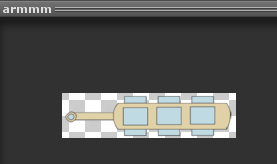
\includegraphics[width=5cm]{03TrabajoRealizado/DocProduccionR/imagenes/n9/n905.png}}
	\subfigure[Imagen de terreno.]{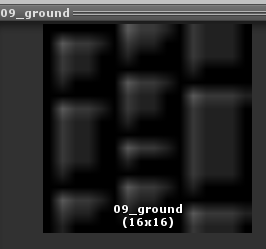
\includegraphics[width=5cm]{03TrabajoRealizado/DocProduccionR/imagenes/n9/n906.png}}
	\caption{Imágenes utilizadas para el nivel} \label{fig:n902}
\end{figure}

Después de reunir los componentes se da a la tarea de dar las acciones que realizarían. En esta parte se omite las plataformas con movimiento tanto horizontal como vertical, pues presentan el mismo comportamiento que los anteriores. También se omite los enemigos fantasmas que ya han sido realizados en los niveles anteriores.

Ya que se tiene los objetos con los comportamientos deseados se procede a ubicarlos según correspondan como se ve en la \ref{fig:n504}.
\begin{figure}
	\centering
	\caption{Maquetado llevado al motor de juego Unity.}
	\label{fig:n504}
	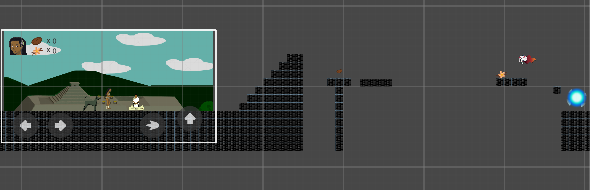
\includegraphics[width=0.5\textwidth]{03TrabajoRealizado/DocProduccionR/imagenes/n9/n902.png}
\end{figure}

Por último se establece las acciones que realiza el jefe enemigo Nexoxcho descritas en la siguiente figura \ref{fig:n905}.
\begin{figure}[htbp]
	\centering
	\subfigure[El jefe enemigo por un cierto tiempo limitado sigue hacia la misma dirección que el jugador, sin importar si es un movimiento horizontal o vertical.]{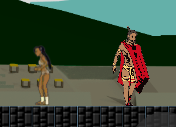
\includegraphics[width=5cm]{03TrabajoRealizado/DocProduccionR/imagenes/n9/n907.png}}
	\subfigure[Después de vencido el tiempo de persecución del jugador, de manera aleatoria realiza un ataque hacia la izquierda o derecha o ambas direcciones.]{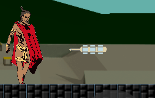
\includegraphics[width=5cm]{03TrabajoRealizado/DocProduccionR/imagenes/n9/n908.png}}
	\caption{Muestra de acciones de el jefe enemigo Nexoxcho.} \label{fig:n905}
\end{figure}
